% based on a template made by the university of cologne
% http://www.mi.uni-koeln.de/wp-MIEDV/wp-content/uploads/2016/07/LaTeX-Vorlage.zip - 2023-11-02
\documentclass[12pt,a4paper]{scrartcl}

\addtokomafont{sectioning}{\rmfamily}
%\usepackage[ngerman]{babel}% deutsches Sprachpaket wird geladen
\usepackage[T1]{fontenc} % westeuropäische Codierung wird verlangt
\usepackage[utf8]{inputenc}% Umlaute werden erlaubt
\usepackage[usenames]{color} % Erlaubt die Benutzung der namen im Farbpaket und deren Änderung
\usepackage{amsmath} % Erweiterung für den Mathe-Satz
\usepackage{amssymb} % alle Zeichen aus msam und msmb werden dargestellt
\usepackage{graphicx} % Graphiken und Bilder können eingebunden werden
%\usepackage{multirow} % erlaubt in einer Spalte einer Tabelle die Felder in mehreren Zeilen zusammenzufassen
\usepackage{enumerate} % erlaubt Nummerierungen
\usepackage{url} % Dient zur Auszeichnung von URLs; setzt die Adresse in Schreibmaschinenschrift.
\usepackage[center]{caption}  % Bildunterschrift wird zentriert
%\usepackage{subfigure} % mehrere Bilder können in einer fugure-Umgebung verwendet werden
%\usepackage{longtable} % Diese Umgebung ist ähnlich definiert wie die tabular-Umgebung, erlaubt jedoch mehrseitige Tabellen.
%\usepackage{paralist} % Modifikation der bereits bestehenden Listenumgebungen
\usepackage{lmodern}% Für die Schrift
\usepackage[hidelinks]{hyperref} % Links und Verweise werden innerhalb von PDF Dokumenten erzeugt
%\usepackage{wrapfig} % Das Paket ermöglicht es von Schrift umflossene Bilder und Tabellen einzufügen.
\usepackage{latexsym} % LaTeX-Symbole werden geladen
\usepackage{tikz} % Erlaubt es mit tikz zu zeichnen
\usepackage{tabularx} % Erlaubt Tabellen
\usepackage{algorithm} % Erlaubt Pseudocode
\usepackage{color} % Farbpaket wird geladen
%\usepackage{stmaryrd} % St Mary Road Symbole werden geladen
\usepackage{physics}

\numberwithin{equation}{section} % Nummerierungen der Gleichungen, die durch equation erstellt werden, sind gebunden an die section
\newcommand{\HRule}{\rule{\linewidth}{0.7mm}}
\newcommand{\pu}[1]{\ensuremath{\mathrm{#1}}}

% disable commands
\renewcommand{\[}{} % math block start
\renewcommand{\]}{\noindent} % math block end
\newcommand{\tightlist}{} % created in enumerations

\hypersetup{
  pdftitle={B 2.5},
  pdfcreator={LaTeX via pandoc}}

\setcounter{secnumdepth}{6}
\setcounter{tocdepth}{6}

\begin{document}
\begin{titlepage}
	\pagestyle{empty}

	\begin{center}

	\textsc{\LARGE Universität zu Köln }\\ [0.4cm]
	\textsc{Mathematisch-Naturwissenschaftliche Fakultät} \\[1.5cm]

	\includegraphics[width=0.45\textwidth]{uni}\\[1.5cm]  % Uni-Logo wird geladen

	\textsc{\Large Praktikum~B}\\[2mm]
	\textsc{}\\[10mm]
	\HRule \\[0.4cm]

		{	\Huge \bfseries B 2.5}\\[0.4cm]
			{	\huge \bfseries Rastertunnelmikroskopie}\\[0.3cm]
	
	\HRule \\[3cm]

			\textsc{\Large Catherine Tran } \\[3pt]
		\textsc{\Large Carlo Kleefisch } \\[3pt]
		\textsc{\Large Oliver Filla } \\[3pt]
		
% 	\begin{center}
% 	\textsc{\Large Catherine~Tran } \\[3pt]
% 	\textsc{\Large Carlo~Kleefisch } \\[3pt]
% 	\textsc{\Large Oliver~Filla } \\[3pt]
% 	\end{center}
	\end{center}
\end{titlepage}

\newpage
\tableofcontents
\newpage

\hypertarget{motivation}{%
\section{Motivation}\label{motivation}}

Mit einem Rastertunnelmikroskop\footnote{engl. Scanning Tunneling
  Microscope (STM)} (STM) können Oberflächenstrukturen in der Größe von
Atomen gemessen werden, wenn die Oberfläche elektrischen Strom leitet.

In diesem Experiment werden zwei verschiedene Proben, eine aus Gold und
eine aus Graphit, vermessen. Als die Graphitprobe wird hochorientiertes
pyrolytisches Graphit (HOPG) verwendet, was eine besonders stabile
Struktur aufweist.

\hypertarget{theoretische-grundlagen}{%
\section{Theoretische Grundlagen}\label{theoretische-grundlagen}}

\hypertarget{tunneleffekt}{%
\subsection{Tunneleffekt}\label{tunneleffekt}}

Quantenmechanische Teilchen können Potentialbarrieren auch dann
überwinden, wenn ihre Energie eigentlich zu niedrig ist. Man spricht
davon, dass sie durch die Barriere hindurchtunneln.

Die tatsächliche Potentialbarriere kann analog zur Gamow-Näherung als
einzelne kastenförmiges Potential \(V(z)\) angenommen werden. Die
Potentialbarriere beginne an der Position \(0\) bei der Probe und Ende
an der Position \(z_0\) an der Messspitze des STMs.

\[
\begin{eqnarray}
    V(z) &=&
        \begin{cases}
            V_0 &: z \in [0, z_0] \\
            0 &: z \notin [0, z_0]
        \end{cases}
\end{eqnarray}
\] Die Lösung der eindimensionalen, stationären Schrödingergleichung
liefert die Tunnelwahrscheinlichkeit \(P(z_0)\), mit der das Teilchen
die Barriere durchtunnelt. Der relevante Parameter \(\kappa\) ist
abhängig von der Elektronenmasse \(m_e\), der Höhe der Potentialbarriere
\(V_0\) und der Energie \(E\) des tunnelnden Elektrons. \(\hbar\) ist
die reduzierte Planck-Konstante.

\[
\begin{eqnarray}
    P(z_0) &\propto& |\Psi(0)|^2 \cdot \mathrm e^{-2\kappa z_0} \\
    \kappa &=& \frac{\sqrt{2m_e(V_0 - E)}}{\hbar} \label{kappa} \\
\end{eqnarray}
\] Diese Wahrscheinlichkeit ist exponentiell von der Breite des
Potentials \(z_0\) abhängig. Zudem ist sie von der Wahrscheinlichkeit
für den Aufenthalt eines Teilchens am Beginn der Probe abhängig, die
durch die quadrierte Wellenfunktion \(|\Psi(0)|^2\).

Diese Wahrscheinlichkeit hängt davon ab, wie wahrscheinlich ein Elektron
aus der Probe austritt. Dazu ist die Austrittsenergie \(\phi\)
essentiell. Dafür wiederum ist die Besetzung der Energieniveaus
relevant, die von der Temperatur und der Fermi-Energie abhängt. Die
Beschreibung erfolgt durch die Zustandsdichte.

Für das STM ist jedoch nicht der Einzelfall interessant, sondern die
Rate, mit der Elektronen aus der Probe austreten und tunneln. Dies kann
durch den \emph{Tunnelstrom} \(I\) beschrieben werden.

Der Tunnelstrom ist proportional zur Tunnelwahrscheinlichkeit
\(P(z_0)\), ebenso zu der Anzahl der Elektronen, die in einer gewissen
Zeit aus dem Material austreten. Dadurch ist der Tunnelstrom
exponentiell von der Breite \(z_0\) der Potentialbarriere abhängig.

\[
\begin{eqnarray}
    I(z_0) &\propto& \mathrm e^{-2\kappa z_0} \label{I(z)}
\end{eqnarray}
\] Durch die exponentielle Abhängigkeit des Tunnelstroms \(I\) von dem
Abstand \(z_0\) ist ein STM sehr sensibel gegen Höhenunterschieden.
Schon ein Höhenunterschied von \(1\,\mathrm{\mathring{A}}\) macht einen
Faktor von näherungsweise \(8\) im Tunnelstrom aus. \([2]\) Dadurch
können Atomstrukturen an der Oberfläche gemessen werden.

\hypertarget{piezoelektrischer-effekt-und-anwendung}{%
\subsection{piezoelektrischer Effekt und
Anwendung}\label{piezoelektrischer-effekt-und-anwendung}}

Der piezoelektrische Effekt bezeichnet die Erzeugung elektrischer
Spannungen an bestimmten Kristallen, den Piezokristallen, bei deren
Deformation. Dies funktioniert auch umgekehrt: Durch Anlegen einer
Spannung verformt sich ein Piezokristall. Dies nennt man \emph{inversen
Piezoeffekt}.

Der inverse Piezoeffekt wird zur Bewegung der Messspitze verwendet.
Diese ist an einer Platform befestigt, die auf drei Piezoröhrchen steht.
Durch Anlegen von Spannung an diesen Röhrchen verformen diese sich. Wird
die Spannung langsam angelegt und plötzlich entfernt, so geschieht diese
Verformung erst langsam, dann sprunghaft.

Wird die Spannung auf diese Weise bei allen drei Piezoröhrchen variiert,
so wird die Position der Messspitze verändert. Hierbei gibt es die zwei
Variationen: Entweder kann die Position auf der Probenoberfläche
verändert werden, beispielsweise kann nach rechts ``gewandert'' werden.
Alternativ kann die Messspitze rotiert werden, ohne die Position auf der
Probenoberfläche zu verändern. Dies kann dazu genutzt werden, um die
Höhe der Messspitze zu steuern.

\hypertarget{gitterstruktur-und-einheitszelle}{%
\subsection{Gitterstruktur und
Einheitszelle}\label{gitterstruktur-und-einheitszelle}}

Was ist eine Einheitszelle? Wie sehen Gitterstrukturen aus?

\hypertarget{durchfuxfchrung}{%
\section{Durchführung}\label{durchfuxfchrung}}

\hypertarget{gold}{%
\subsection{Gold}\label{gold}}

\hypertarget{strukturmessung}{%
\subsubsection{Strukturmessung}\label{strukturmessung}}

Zunächst wird die grobe Struktur von Gold gemessen, dabei wird eine
Stufenkante gesucht. Dies erweist sich als schwierig, da die Probe
kontaminiert ist. Es entstehen keine scharfen Bilder, allerdings gibt es
eine Stelle mit mehreren scharfen Kanten. Diese sehen jedoch nicht nach
Gold aus, vermutlich wurde ein Fremdkörper vermessen.

Die Probe ist zerkratzt, dies ist mit dem bloßen Auge sichtbar. Andere
Kontaminationen, u.a. biologischer Natur, werden explizit nicht
ausgeschlossen.

\hypertarget{austrittsarbeit}{%
\subsubsection{Austrittsarbeit}\label{austrittsarbeit}}

Zur Messung der Austrittsarbeit wird die Messspitze an der selben
Position in der Höhe verändert, dabei wird der Tunnelstrom \(I(z)\)
gemessen. Im ersten Teil wird sie um \(3\,\mathrm{\mathring{A}}\)
abgesenkt und wieder angehoben, im zweiten Teil wird die Messspitze
stattdessen um \(3\,\mathrm{\mathring{A}}\) angehoben und wieder
abgesenkt.

\hypertarget{graphit}{%
\subsection{Graphit}\label{graphit}}

Wie bei der Goldprobe wird zunächst ein grobes Bild der Struktur
gemessen. Dabei soll eine glatte Stelle gefunden werden, an der eine
Detailaufnahme der Atomstruktur aufgenommen wird. Wie auch die Goldprobe
ist auch diese Probe zerkratzt, was wieder mit bloßem Auge zu erkennen
ist.

\hypertarget{auswertung}{%
\section{Auswertung}\label{auswertung}}

Die Messergebnisse können mit der Software
\href{http://gwyddion.net}{Gwyddion} \([1]\) alternativ mit
\href{http://www.wsxm.eu}{WSxM} \([2]\) ausgewertet werden.

\hypertarget{gold-1}{%
\subsection{Gold}\label{gold-1}}

Die im Versuch aufgenommenen Bilder von Gold sind alle sehr verschieden.
Auf einigen ist das Rauschen zu groß und es sind amorphe Region zu
sehen, deshalb werden sie nicht im Protokoll weiter diskutiert. Daher
wurden uns vonseiten der Versuchsbetreung zusätzliche Daten zur
Auswertung bereitgestellt. \([6]\)

\hypertarget{eigene-messung}{%
\subsubsection{eigene Messung}\label{eigene-messung}}

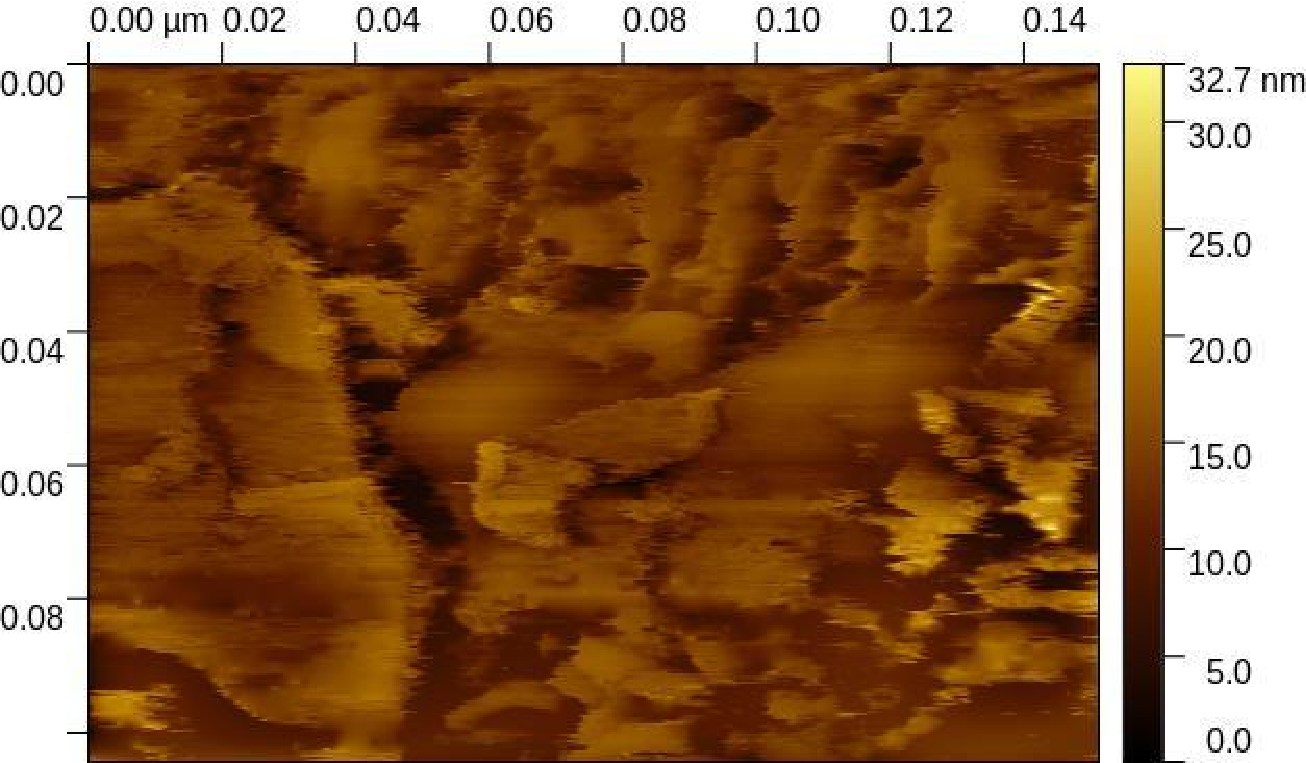
\includegraphics{Gold_gross.pdf} In Abbildung 1?? kann man mögliche
Stufenkanten sehen. Das darunterliegende Gebiet ist nicht eindeutig zu
identifizieren. Vermutlich erstrecken sich viele Stufenkanten über
diesem Bild, was aber wegen Rauschen im Messsignal unklar ist.

Die gesamte Struktur sieht nicht nach einem Einkristall aus. Dies legt
die Vermutung nahe, dass Fremdkörper auf der Probe sind.

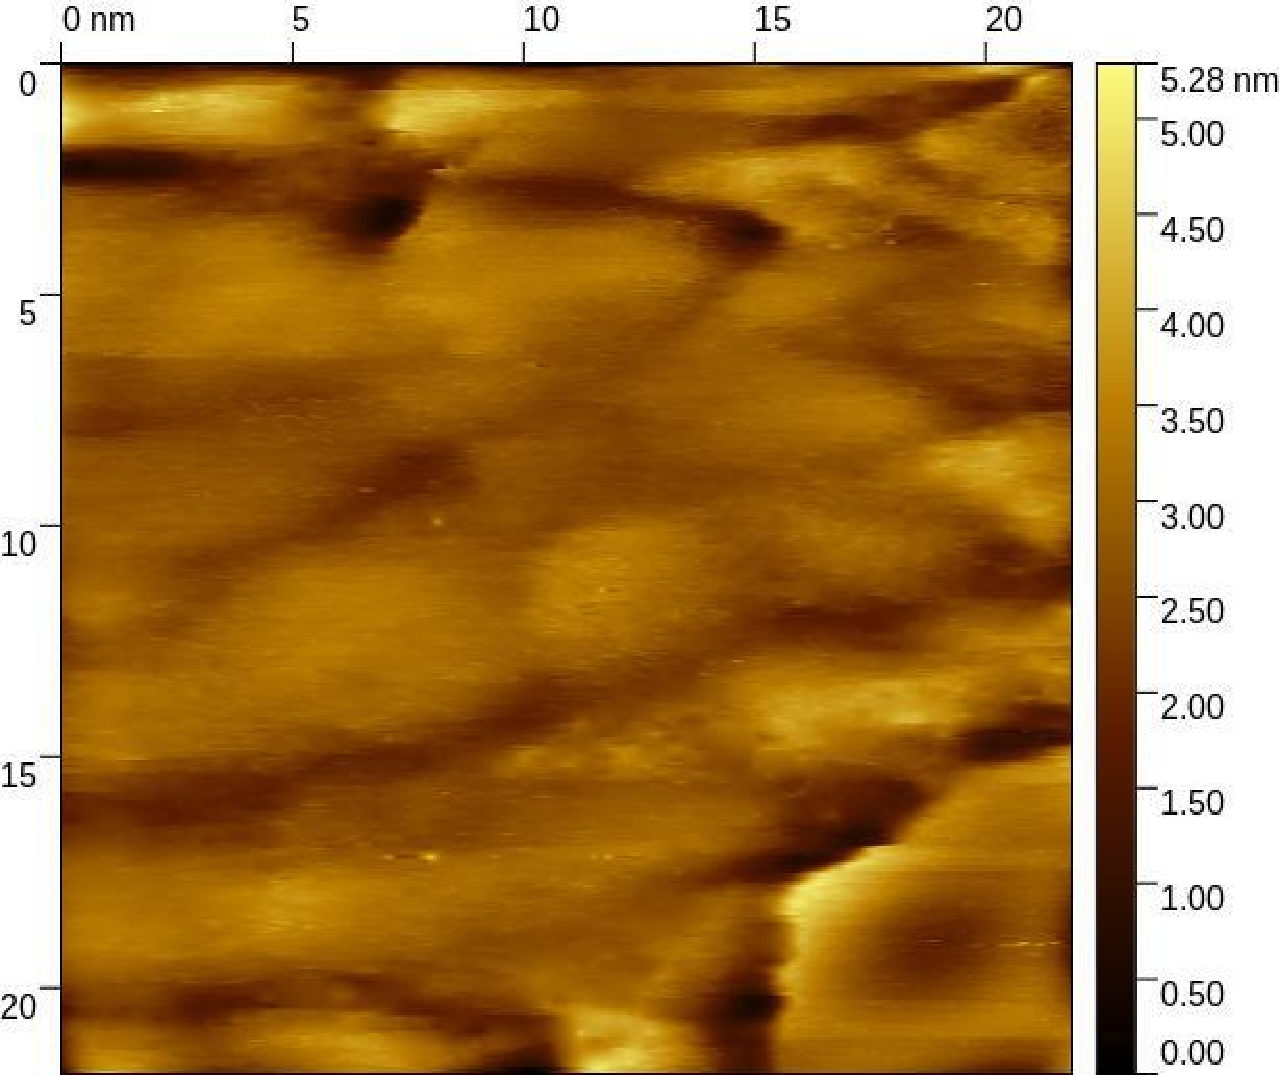
\includegraphics{Gold_Stufenkante.pdf} Bei Abbildung 2?? erkennt man
eine mögliche Terrassenstruktur, die von links nach rechts verlaufen.
Auch hier leiden die Bilddetails unter der schlechten Qualität, scharfe
Kanten sind nicht zu erkennen. Möglicherweise gibt es auch hier
Fremdstoffe, die z.B. die Leitfähigkeit oder die
Tunnelwahrscheinlichkeit beeinflussen.

Biologisches Material wie Fettspuren könnten diese Bilder erklären.

\hypertarget{bereitgestelltes-material}{%
\subsubsection{bereitgestelltes
Material}\label{bereitgestelltes-material}}

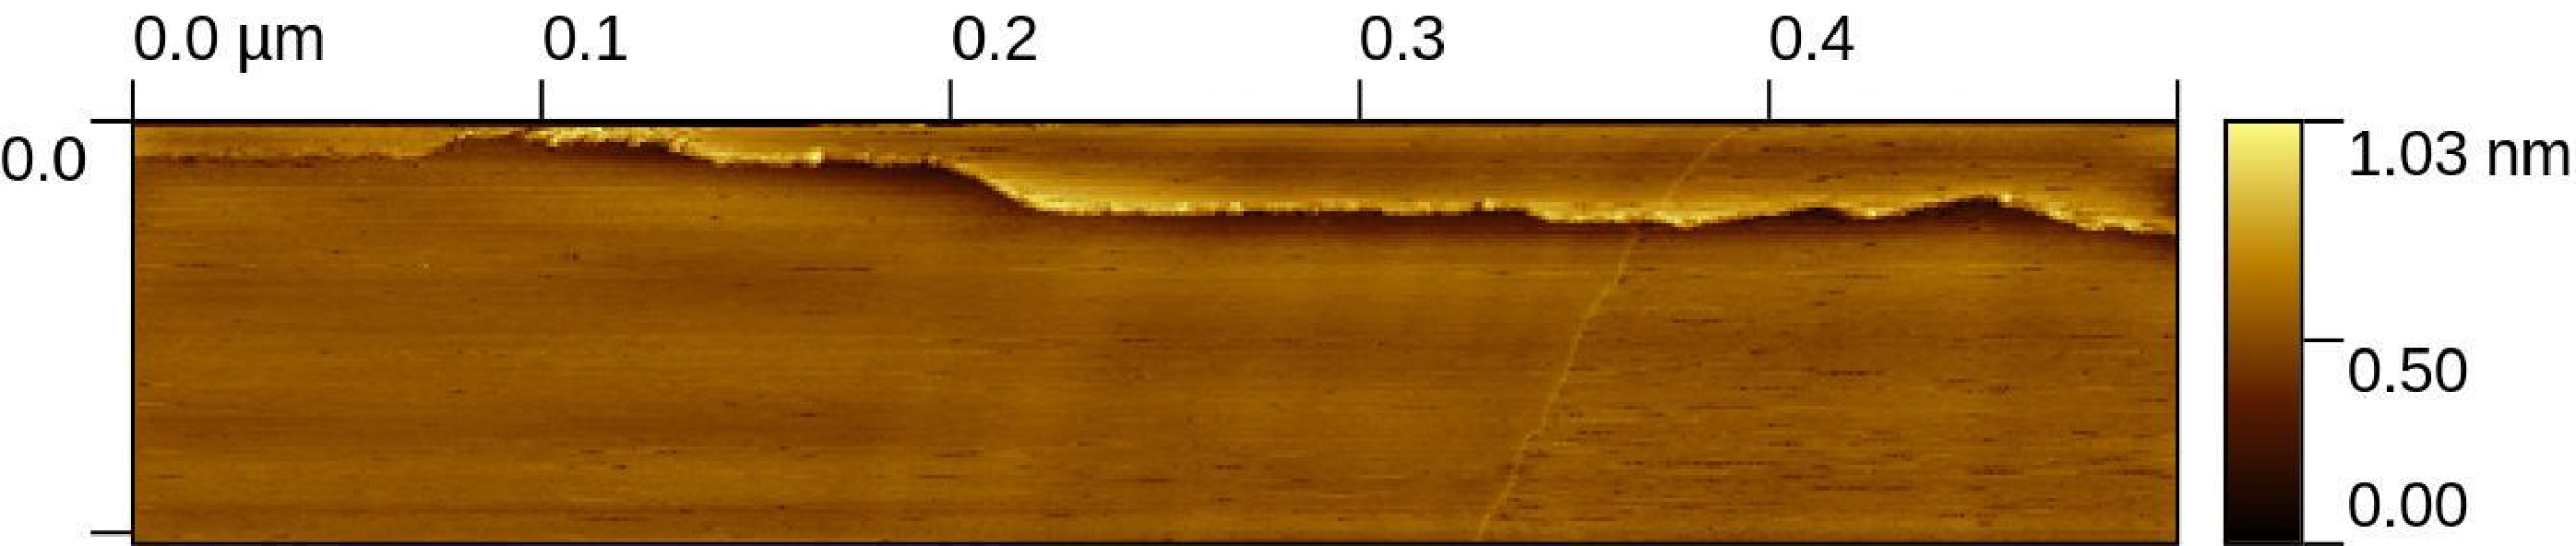
\includegraphics{Stufenkante.pdf} In Abbildung 3?? kann man eine
Stufenkante in der Höhe von \(1.03\mathrm{\,nm}\) in der oberen rechten
Bildhälfte erkennen. Die Oberfläche scheint sehr glatt zu sein, wobei
auch hier ein Rauschen im Bild auftritt.

Die Stufenkante entsteht bei der Abkühlung nach dem Ausglühen der Probe,
d.h. durch die thermische Spannung. Gold besitzt eine
\(\mathrm{fcc}\)-Gitterstruktur, so treten die Stufenversetzungen in den
\(\braket{111}\)-Ebenen auf, die sind auch die dichtgepackten Ebenen
sind. Die Stufenkante verläuft in die selbe Richtung wie der
Burgersvektor, nämlich in die \(\braket{110}\)-Richtungen.

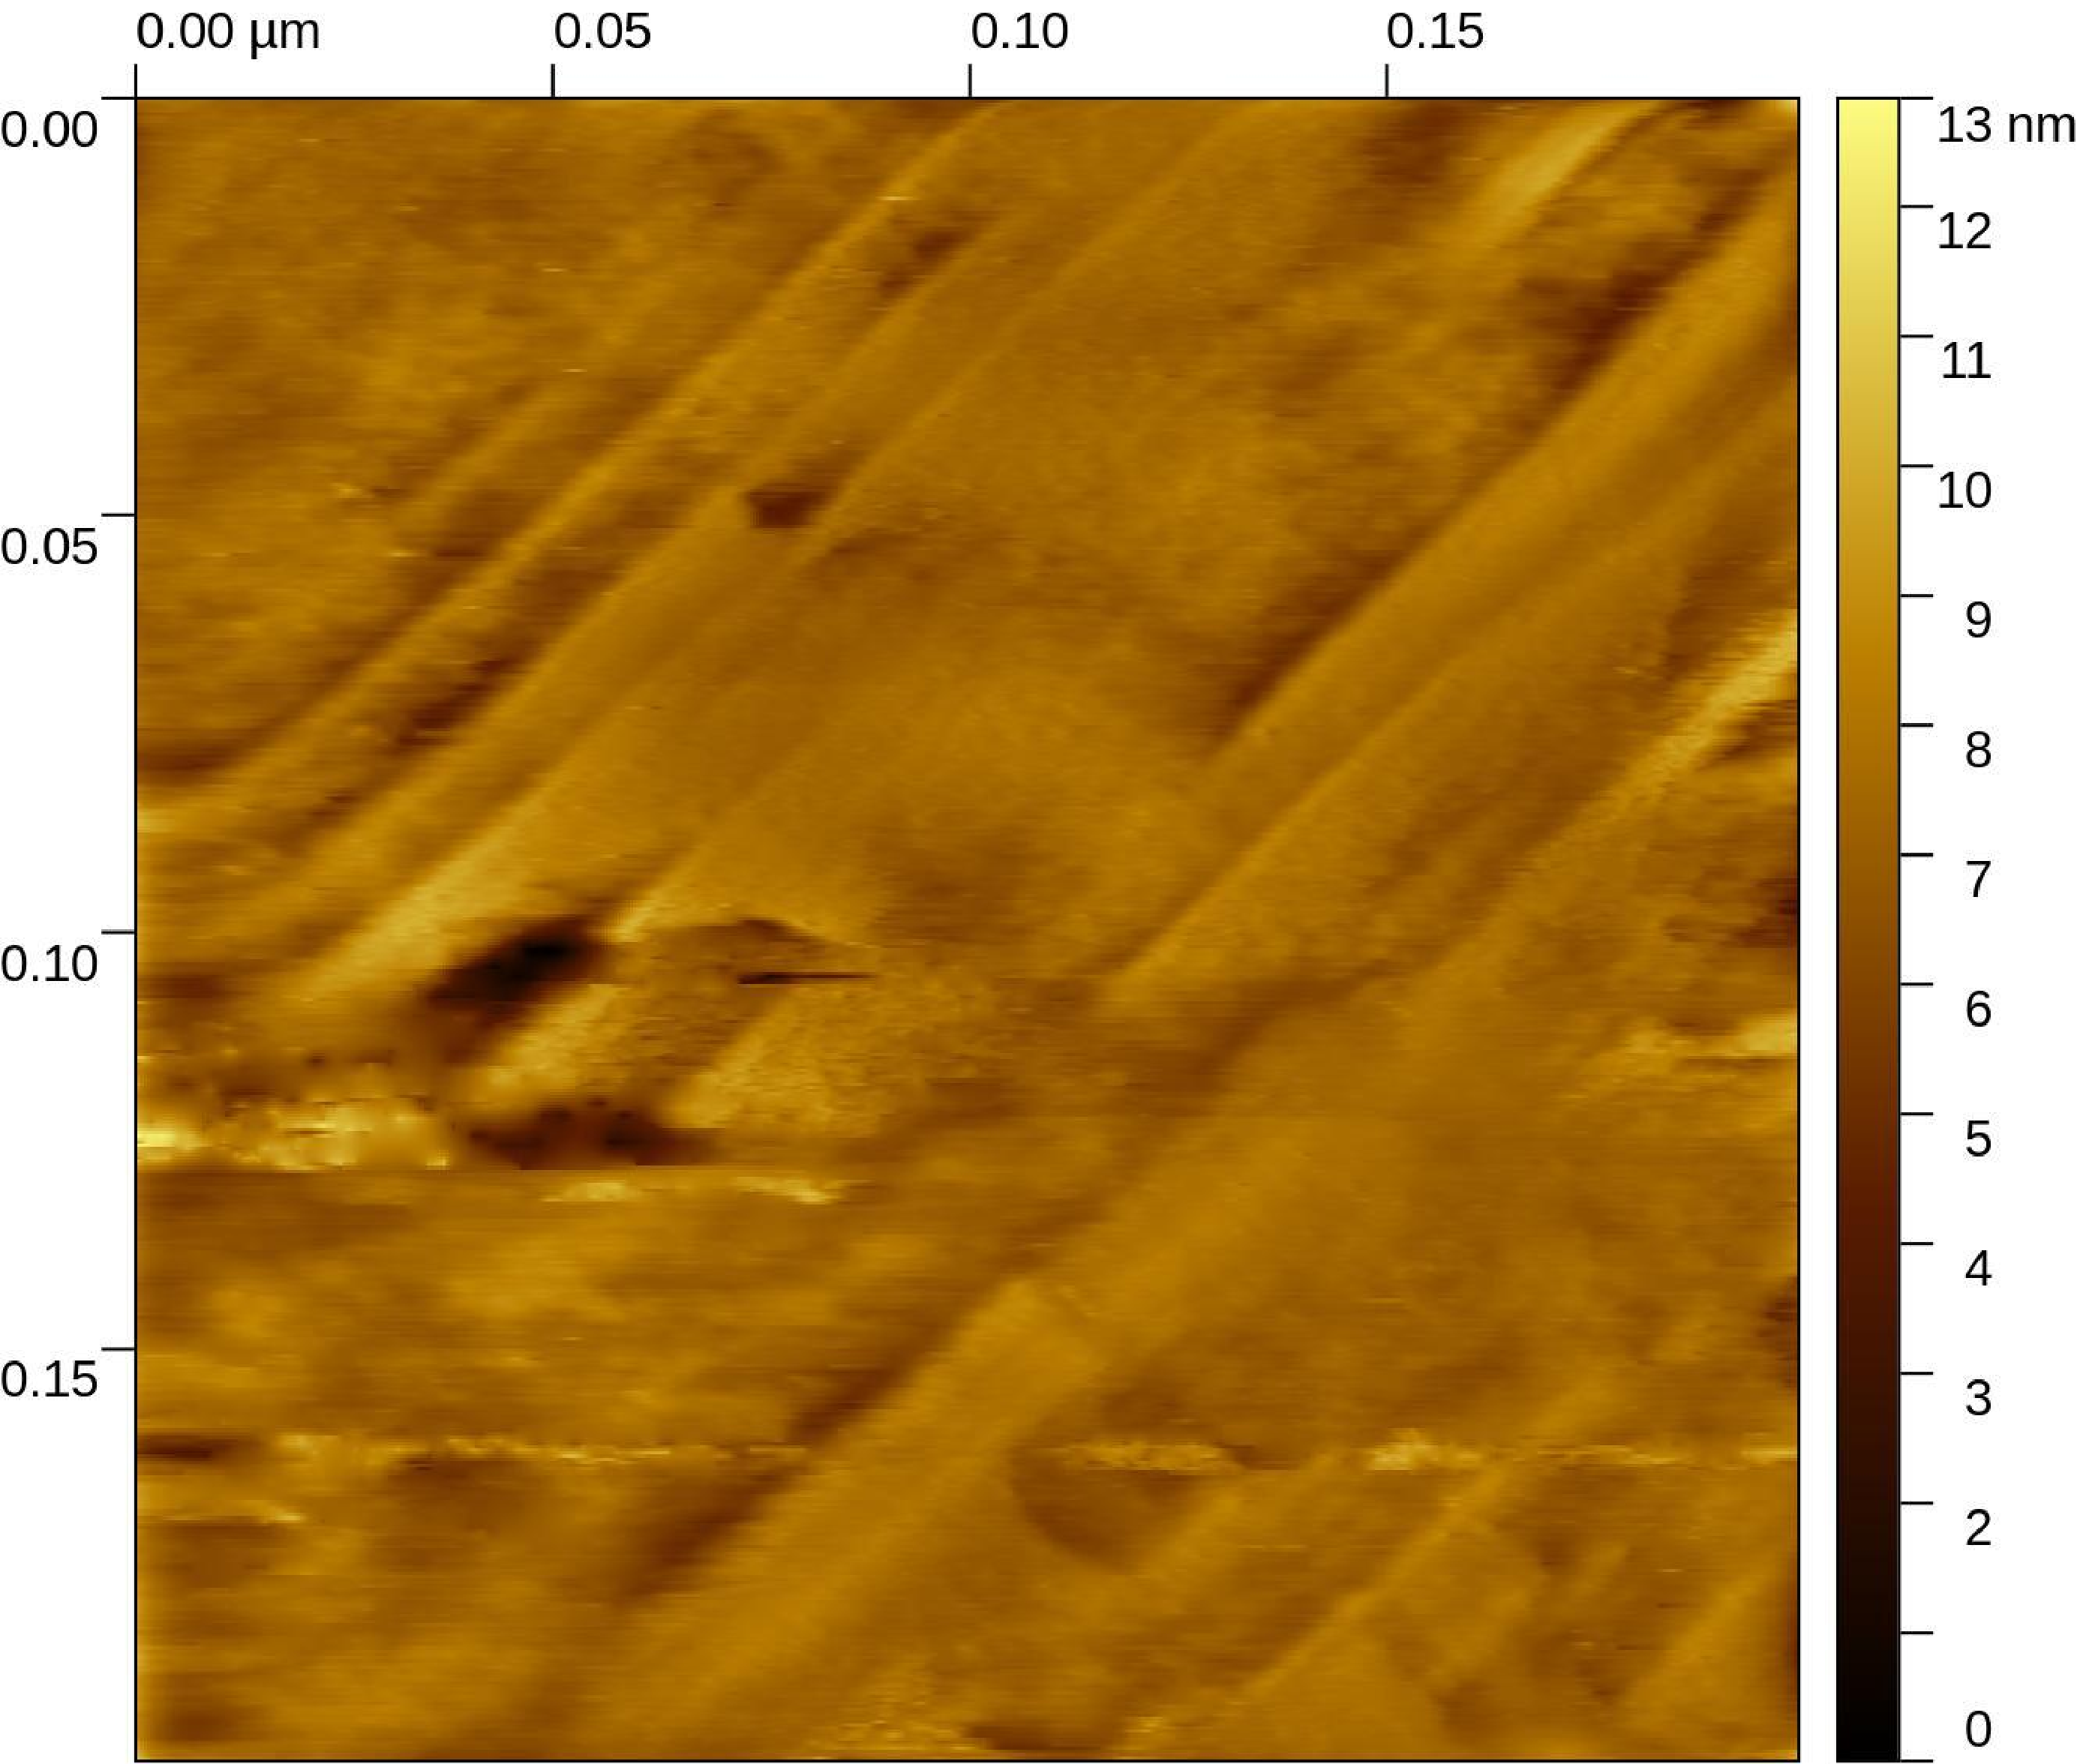
\includegraphics{Gold.pdf} In Abbildung 4?? sind Terrassen abgebildet,
die von Stufenkanten getrennt sind. Die Stufen verlaufen von unten
rechts nach oben links und die Breite der einzelnen Stufen scheinen
relativ gleichmäßig zu sein.

\hypertarget{vergleich}{%
\subsubsection{Vergleich}\label{vergleich}}

Die von uns erstellten Messungen unterscheiden sich massiv von den
bereitgestellten Messungen. Alle Messungen haben eine vergleichbare
Bias-Spannung, die Stromstärken unterscheiden sich jedoch.

Insbesondere die bereitgestellte Messung der Stufenkante (Abb. 3??) ist
bei einer deutlich geringeren Stromstärke als alle anderen Messungen an
Gold vorgenommen worden, die Stromstärken unterscheiden sich um einen
Faktor \(6\) von unseren Stromstärken. Die Stromstärken von unseren
Messungen sind jedoch auch um ca. \(30\%\) größer als die
bereitgestellte Messung der Terassen (Abb. 4??) bei
\(3.5 \mathrm{\,nA}\). Dies unterstützt die These, dass unsere Probe
nicht sauber ist und eine Barriere aus Fremdstoffen die
Tunnelwahrscheinlichkeit verringert.

\hypertarget{austrittsarbeit-1}{%
\subsubsection{Austrittsarbeit}\label{austrittsarbeit-1}}

Die Austrittsarbeit \(\phi\) ist die Differenz zwischen
Potentialbarriere \(V_0\) und der Energie \(E\) der tunnelnden
Elektronen. Mithilfe der Relationen für die Tunnelwahrscheinlichkeit
\(\eqref{kappa}\) und den Tunnelstrom \(\eqref{I(z)}\) kann man die
Austrittsarbeit ermitteln.

\[
\begin{eqnarray}
    I(z) &\propto& \exp\left[-2\frac{\sqrt{2m_e\cdot \phi}}{\hbar} z\right] \\
    \ln\eqref{I(z)}
        &=& \ln(c)
            + \left(-2\frac{\sqrt{2m_e}}{\hbar}\right)
            \cdot \sqrt{\phi} \cdot z \\
    \ln\eqref{I(z)} &=& \ln(c) + 0.51 \mathrm{\,\frac{\sqrt{eV}}{\mathrm{\mathring{A}}}}\cdot \sqrt{\phi} \cdot z
\end{eqnarray}
\] Im letzten Schritt wurden die Naturkonstanten passend eingesetzt.
\([3]\) Dadurch kann die Austrittsarbeit aus der Steigung \(m\) einer
Regression von \(\ln\eqref{I(z)}\) ermittelt werden.

\[
\begin{eqnarray}
    \phi &=& \left(\frac{m}{0.51}\right)^2 \mathrm{\,eV}
\end{eqnarray}
\]

Dadurch ergeben sich folgende Ergebnisse, von denen die erste Hälfte aus
der ersten Messung und die zweite Hälfte aus der zweiten Messung
stammen.

\[
\begin{align*}
    \text{Steigung } m &\text{ in } 10^{-3}\mathrm{\mathring A}^{-1}
        & \phi &\text{ in } 10^{-6}\mathrm{eV} \\
    10.549 &\pm 0.049 & 111.290 &\pm 0.002 \\
    16.579 &\pm 0.079 & 274.872 &\pm 0.006 \\
    16.464 &\pm 0.078 & 271.057 &\pm 0.006 \\
    15.579 &\pm 0.065 & 242.699 &\pm 0.004 \\
    17.176 &\pm 0.054 & 295.018 &\pm 0.003 \\
    12.439 &\pm 0.048 & 154.737 &\pm 0.002 \\
    10.123 &\pm 0.038 & 102.478 &\pm 0.001 \\
    13.417 &\pm 0.043 & 180.009 &\pm 0.002 \\
    13.945 &\pm 0.038 & 194.458 &\pm 0.001 \\
    13.526 &\pm 0.057 & 182.949 &\pm 0.003 
\end{align*}
\] \# Fazit \# Literatur 1. Gwyddion, \url{http://gwyddion.net} 2. I.
Horcas, R. Fernandez, J.M. Gomez-Rodriguez, J. Colchero, J.
Gomez-Herrero and A. M. Baro, Rev.~Sci. Instrum. 78, 013705 (2007),
\url{http://www.wsxm.eu} 3. Universität zu Köln, ``Versuch B.2.5.
Rastertunnelmikroskopie'', 31.03.2017,
\url{https://ph2.uni-koeln.de/fileadmin/Lehre/PraktikumB/B2.5_Anleitung_2017_03.pdf}
4. H. A. Mizes, W. A. Harrison und S.-i. Park, ``Multiple-tip
interpretation of anomalous scanning-tunneling-microscopy images of
layered materials'', Physical Review B Volume 36, pp.~4491 - 4494, 15.
September 1987 5. H. J. Mamin, E. Ganz, D. W. Abraham, R. E. Thomson und
J. Clarke, ``Contamination- mediated deformation of graphite by the
scanning tunneling microscope'', Physical Review B Volume 34, 15.
Dezember 1986 6. Versuchsbetreuung: M.Sc. Catherine Grover, Studentin
der Festkörperphysik im PhD an der Universität zu Köln,
\url{https://ph2.uni-koeln.de/en/research-groups/group-michely/members}

\end{document}
